% Options for packages loaded elsewhere
\PassOptionsToPackage{unicode}{hyperref}
\PassOptionsToPackage{hyphens}{url}
\PassOptionsToPackage{dvipsnames,svgnames,x11names}{xcolor}
%
\documentclass[
  letterpaper,
  DIV=11,
  numbers=noendperiod]{scrartcl}

\usepackage{amsmath,amssymb}
\usepackage{iftex}
\ifPDFTeX
  \usepackage[T1]{fontenc}
  \usepackage[utf8]{inputenc}
  \usepackage{textcomp} % provide euro and other symbols
\else % if luatex or xetex
  \usepackage{unicode-math}
  \defaultfontfeatures{Scale=MatchLowercase}
  \defaultfontfeatures[\rmfamily]{Ligatures=TeX,Scale=1}
\fi
\usepackage{lmodern}
\ifPDFTeX\else  
    % xetex/luatex font selection
\fi
% Use upquote if available, for straight quotes in verbatim environments
\IfFileExists{upquote.sty}{\usepackage{upquote}}{}
\IfFileExists{microtype.sty}{% use microtype if available
  \usepackage[]{microtype}
  \UseMicrotypeSet[protrusion]{basicmath} % disable protrusion for tt fonts
}{}
\makeatletter
\@ifundefined{KOMAClassName}{% if non-KOMA class
  \IfFileExists{parskip.sty}{%
    \usepackage{parskip}
  }{% else
    \setlength{\parindent}{0pt}
    \setlength{\parskip}{6pt plus 2pt minus 1pt}}
}{% if KOMA class
  \KOMAoptions{parskip=half}}
\makeatother
\usepackage{xcolor}
\setlength{\emergencystretch}{3em} % prevent overfull lines
\setcounter{secnumdepth}{-\maxdimen} % remove section numbering
% Make \paragraph and \subparagraph free-standing
\makeatletter
\ifx\paragraph\undefined\else
  \let\oldparagraph\paragraph
  \renewcommand{\paragraph}{
    \@ifstar
      \xxxParagraphStar
      \xxxParagraphNoStar
  }
  \newcommand{\xxxParagraphStar}[1]{\oldparagraph*{#1}\mbox{}}
  \newcommand{\xxxParagraphNoStar}[1]{\oldparagraph{#1}\mbox{}}
\fi
\ifx\subparagraph\undefined\else
  \let\oldsubparagraph\subparagraph
  \renewcommand{\subparagraph}{
    \@ifstar
      \xxxSubParagraphStar
      \xxxSubParagraphNoStar
  }
  \newcommand{\xxxSubParagraphStar}[1]{\oldsubparagraph*{#1}\mbox{}}
  \newcommand{\xxxSubParagraphNoStar}[1]{\oldsubparagraph{#1}\mbox{}}
\fi
\makeatother

\usepackage{color}
\usepackage{fancyvrb}
\newcommand{\VerbBar}{|}
\newcommand{\VERB}{\Verb[commandchars=\\\{\}]}
\DefineVerbatimEnvironment{Highlighting}{Verbatim}{commandchars=\\\{\}}
% Add ',fontsize=\small' for more characters per line
\usepackage{framed}
\definecolor{shadecolor}{RGB}{241,243,245}
\newenvironment{Shaded}{\begin{snugshade}}{\end{snugshade}}
\newcommand{\AlertTok}[1]{\textcolor[rgb]{0.68,0.00,0.00}{#1}}
\newcommand{\AnnotationTok}[1]{\textcolor[rgb]{0.37,0.37,0.37}{#1}}
\newcommand{\AttributeTok}[1]{\textcolor[rgb]{0.40,0.45,0.13}{#1}}
\newcommand{\BaseNTok}[1]{\textcolor[rgb]{0.68,0.00,0.00}{#1}}
\newcommand{\BuiltInTok}[1]{\textcolor[rgb]{0.00,0.23,0.31}{#1}}
\newcommand{\CharTok}[1]{\textcolor[rgb]{0.13,0.47,0.30}{#1}}
\newcommand{\CommentTok}[1]{\textcolor[rgb]{0.37,0.37,0.37}{#1}}
\newcommand{\CommentVarTok}[1]{\textcolor[rgb]{0.37,0.37,0.37}{\textit{#1}}}
\newcommand{\ConstantTok}[1]{\textcolor[rgb]{0.56,0.35,0.01}{#1}}
\newcommand{\ControlFlowTok}[1]{\textcolor[rgb]{0.00,0.23,0.31}{\textbf{#1}}}
\newcommand{\DataTypeTok}[1]{\textcolor[rgb]{0.68,0.00,0.00}{#1}}
\newcommand{\DecValTok}[1]{\textcolor[rgb]{0.68,0.00,0.00}{#1}}
\newcommand{\DocumentationTok}[1]{\textcolor[rgb]{0.37,0.37,0.37}{\textit{#1}}}
\newcommand{\ErrorTok}[1]{\textcolor[rgb]{0.68,0.00,0.00}{#1}}
\newcommand{\ExtensionTok}[1]{\textcolor[rgb]{0.00,0.23,0.31}{#1}}
\newcommand{\FloatTok}[1]{\textcolor[rgb]{0.68,0.00,0.00}{#1}}
\newcommand{\FunctionTok}[1]{\textcolor[rgb]{0.28,0.35,0.67}{#1}}
\newcommand{\ImportTok}[1]{\textcolor[rgb]{0.00,0.46,0.62}{#1}}
\newcommand{\InformationTok}[1]{\textcolor[rgb]{0.37,0.37,0.37}{#1}}
\newcommand{\KeywordTok}[1]{\textcolor[rgb]{0.00,0.23,0.31}{\textbf{#1}}}
\newcommand{\NormalTok}[1]{\textcolor[rgb]{0.00,0.23,0.31}{#1}}
\newcommand{\OperatorTok}[1]{\textcolor[rgb]{0.37,0.37,0.37}{#1}}
\newcommand{\OtherTok}[1]{\textcolor[rgb]{0.00,0.23,0.31}{#1}}
\newcommand{\PreprocessorTok}[1]{\textcolor[rgb]{0.68,0.00,0.00}{#1}}
\newcommand{\RegionMarkerTok}[1]{\textcolor[rgb]{0.00,0.23,0.31}{#1}}
\newcommand{\SpecialCharTok}[1]{\textcolor[rgb]{0.37,0.37,0.37}{#1}}
\newcommand{\SpecialStringTok}[1]{\textcolor[rgb]{0.13,0.47,0.30}{#1}}
\newcommand{\StringTok}[1]{\textcolor[rgb]{0.13,0.47,0.30}{#1}}
\newcommand{\VariableTok}[1]{\textcolor[rgb]{0.07,0.07,0.07}{#1}}
\newcommand{\VerbatimStringTok}[1]{\textcolor[rgb]{0.13,0.47,0.30}{#1}}
\newcommand{\WarningTok}[1]{\textcolor[rgb]{0.37,0.37,0.37}{\textit{#1}}}

\providecommand{\tightlist}{%
  \setlength{\itemsep}{0pt}\setlength{\parskip}{0pt}}\usepackage{longtable,booktabs,array}
\usepackage{calc} % for calculating minipage widths
% Correct order of tables after \paragraph or \subparagraph
\usepackage{etoolbox}
\makeatletter
\patchcmd\longtable{\par}{\if@noskipsec\mbox{}\fi\par}{}{}
\makeatother
% Allow footnotes in longtable head/foot
\IfFileExists{footnotehyper.sty}{\usepackage{footnotehyper}}{\usepackage{footnote}}
\makesavenoteenv{longtable}
\usepackage{graphicx}
\makeatletter
\def\maxwidth{\ifdim\Gin@nat@width>\linewidth\linewidth\else\Gin@nat@width\fi}
\def\maxheight{\ifdim\Gin@nat@height>\textheight\textheight\else\Gin@nat@height\fi}
\makeatother
% Scale images if necessary, so that they will not overflow the page
% margins by default, and it is still possible to overwrite the defaults
% using explicit options in \includegraphics[width, height, ...]{}
\setkeys{Gin}{width=\maxwidth,height=\maxheight,keepaspectratio}
% Set default figure placement to htbp
\makeatletter
\def\fps@figure{htbp}
\makeatother

\KOMAoption{captions}{tableheading}
\makeatletter
\@ifpackageloaded{caption}{}{\usepackage{caption}}
\AtBeginDocument{%
\ifdefined\contentsname
  \renewcommand*\contentsname{Table of contents}
\else
  \newcommand\contentsname{Table of contents}
\fi
\ifdefined\listfigurename
  \renewcommand*\listfigurename{List of Figures}
\else
  \newcommand\listfigurename{List of Figures}
\fi
\ifdefined\listtablename
  \renewcommand*\listtablename{List of Tables}
\else
  \newcommand\listtablename{List of Tables}
\fi
\ifdefined\figurename
  \renewcommand*\figurename{Figure}
\else
  \newcommand\figurename{Figure}
\fi
\ifdefined\tablename
  \renewcommand*\tablename{Table}
\else
  \newcommand\tablename{Table}
\fi
}
\@ifpackageloaded{float}{}{\usepackage{float}}
\floatstyle{ruled}
\@ifundefined{c@chapter}{\newfloat{codelisting}{h}{lop}}{\newfloat{codelisting}{h}{lop}[chapter]}
\floatname{codelisting}{Listing}
\newcommand*\listoflistings{\listof{codelisting}{List of Listings}}
\makeatother
\makeatletter
\makeatother
\makeatletter
\@ifpackageloaded{caption}{}{\usepackage{caption}}
\@ifpackageloaded{subcaption}{}{\usepackage{subcaption}}
\makeatother

\ifLuaTeX
  \usepackage{selnolig}  % disable illegal ligatures
\fi
\usepackage{bookmark}

\IfFileExists{xurl.sty}{\usepackage{xurl}}{} % add URL line breaks if available
\urlstyle{same} % disable monospaced font for URLs
\hypersetup{
  pdftitle={Class 9: Structural Bioinformatics pt.1},
  pdfauthor={Noel Lim (PID: A17652474)},
  colorlinks=true,
  linkcolor={blue},
  filecolor={Maroon},
  citecolor={Blue},
  urlcolor={Blue},
  pdfcreator={LaTeX via pandoc}}


\title{Class 9: Structural Bioinformatics pt.1}
\author{Noel Lim (PID: A17652474)}
\date{}

\begin{document}
\maketitle


The main database for structural data is called the PBD (Protein Data
Bank). Let's see what it contains:

Data from: https://www.rcsb.com/stats

Read this into R

\begin{Shaded}
\begin{Highlighting}[]
\NormalTok{pdbdb }\OtherTok{\textless{}{-}} \FunctionTok{read.csv}\NormalTok{(}\StringTok{"Data Export Summary.csv"}\NormalTok{)}
\end{Highlighting}
\end{Shaded}

and answer the following questions:

\begin{quote}
Q1: What percentage of structures in the PDB are solved by X-Ray and
Electron Microscopy.
\end{quote}

\begin{Shaded}
\begin{Highlighting}[]
\NormalTok{pdbdb}\SpecialCharTok{$}\NormalTok{Total}
\end{Highlighting}
\end{Shaded}

\begin{verbatim}
[1] "195,866" "12,328"  "13,746"  "4,532"   "213"     "22"     
\end{verbatim}

I need to remove the comma and convert to numeric to do math:

\begin{Shaded}
\begin{Highlighting}[]
\FunctionTok{as.numeric}\NormalTok{( }\FunctionTok{sub}\NormalTok{(}\StringTok{","}\NormalTok{,}\StringTok{""}\NormalTok{, pdbdb}\SpecialCharTok{$}\NormalTok{Total) )}
\end{Highlighting}
\end{Shaded}

\begin{verbatim}
[1] 195866  12328  13746   4532    213     22
\end{verbatim}

I could turn this into a function to fix the whole table or any future
table I read like this:

\begin{Shaded}
\begin{Highlighting}[]
\NormalTok{x }\OtherTok{\textless{}{-}}\NormalTok{ pdbdb}\SpecialCharTok{$}\NormalTok{Total}
\FunctionTok{as.numeric}\NormalTok{( }\FunctionTok{sub}\NormalTok{(}\StringTok{","}\NormalTok{,}\StringTok{""}\NormalTok{,x))}
\end{Highlighting}
\end{Shaded}

\begin{verbatim}
[1] 195866  12328  13746   4532    213     22
\end{verbatim}

\begin{Shaded}
\begin{Highlighting}[]
\NormalTok{comma2numeric }\OtherTok{\textless{}{-}} \ControlFlowTok{function}\NormalTok{(x) \{}
  \FunctionTok{as.numeric}\NormalTok{( }\FunctionTok{sub}\NormalTok{(}\StringTok{","}\NormalTok{,}\StringTok{""}\NormalTok{, x))}
\NormalTok{\}}
\end{Highlighting}
\end{Shaded}

Test it

\begin{Shaded}
\begin{Highlighting}[]
\FunctionTok{comma2numeric}\NormalTok{(pdbdb}\SpecialCharTok{$}\NormalTok{X.ray)}
\end{Highlighting}
\end{Shaded}

\begin{verbatim}
[1] 167317   9645   8735   2869    170     11
\end{verbatim}

\begin{Shaded}
\begin{Highlighting}[]
\FunctionTok{apply}\NormalTok{(pdbdb, }\DecValTok{2}\NormalTok{, comma2numeric)}
\end{Highlighting}
\end{Shaded}

\begin{verbatim}
Warning in FUN(newX[, i], ...): NAs introduced by coercion
\end{verbatim}

\begin{verbatim}
     Molecular.Type  X.ray    EM   NMR Multiple.methods Neutron Other  Total
[1,]             NA 167317 15698 12534              208      77    32 195866
[2,]             NA   9645  2639    34                8       2     0  12328
[3,]             NA   8735  4718   286                7       0     0  13746
[4,]             NA   2869   138  1507               14       3     1   4532
[5,]             NA    170    10    33                0       0     0    213
[6,]             NA     11     0     6                1       0     4     22
\end{verbatim}

\subsection{Or try a different read/import
function:}\label{or-try-a-different-readimport-function}

\begin{Shaded}
\begin{Highlighting}[]
\FunctionTok{library}\NormalTok{(readr)}
\NormalTok{pdbdb }\OtherTok{\textless{}{-}} \FunctionTok{read\_csv}\NormalTok{(}\StringTok{"Data Export Summary.csv"}\NormalTok{)}
\end{Highlighting}
\end{Shaded}

\begin{verbatim}
Rows: 6 Columns: 8
-- Column specification --------------------------------------------------------
Delimiter: ","
chr (1): Molecular Type
dbl (3): Multiple methods, Neutron, Other
num (4): X-ray, EM, NMR, Total

i Use `spec()` to retrieve the full column specification for this data.
i Specify the column types or set `show_col_types = FALSE` to quiet this message.
\end{verbatim}

\begin{Shaded}
\begin{Highlighting}[]
\FunctionTok{sum}\NormalTok{(pdbdb}\SpecialCharTok{$}\NormalTok{Total)}
\end{Highlighting}
\end{Shaded}

\begin{verbatim}
[1] 226707
\end{verbatim}

\begin{Shaded}
\begin{Highlighting}[]
\FunctionTok{sum}\NormalTok{(pdbdb}\SpecialCharTok{$}\StringTok{\textasciigrave{}}\AttributeTok{X{-}ray}\StringTok{\textasciigrave{}}\NormalTok{)}\SpecialCharTok{/}\FunctionTok{sum}\NormalTok{(pdbdb}\SpecialCharTok{$}\NormalTok{Total) }\SpecialCharTok{*} \DecValTok{100}
\end{Highlighting}
\end{Shaded}

\begin{verbatim}
[1] 83.25592
\end{verbatim}

\begin{Shaded}
\begin{Highlighting}[]
\FunctionTok{sum}\NormalTok{(pdbdb}\SpecialCharTok{$}\NormalTok{EM)}\SpecialCharTok{/}\FunctionTok{sum}\NormalTok{(pdbdb}\SpecialCharTok{$}\NormalTok{Total) }\SpecialCharTok{*} \DecValTok{100}
\end{Highlighting}
\end{Shaded}

\begin{verbatim}
[1] 10.2348
\end{verbatim}

\begin{quote}
Q2: What proportion of structures in the PDB are protein?
\end{quote}

\begin{Shaded}
\begin{Highlighting}[]
\NormalTok{pdbdb}\SpecialCharTok{$}\NormalTok{Total[}\DecValTok{1}\NormalTok{]}\SpecialCharTok{/} \FunctionTok{sum}\NormalTok{(pdbdb}\SpecialCharTok{$}\NormalTok{Total) }\SpecialCharTok{*} \DecValTok{100}
\end{Highlighting}
\end{Shaded}

\begin{verbatim}
[1] 86.3961
\end{verbatim}

\begin{quote}
Q3: Type HIV in the PDB website search box on the home page and
determine how many HIV-1 protease structures are in the current PDB?
\end{quote}

\subsection{Mol*}\label{mol}

Mol* (pronounced ``molstar'') is a new web-based molecular viewer than
we will need to learn the basics of here.

https://molstar.org/viewer/

We will use PDB code: 1HSG

\begin{figure}[H]

{\centering \includegraphics{1HSG1.png}

}

\caption{First image from the start}

\end{figure}%

Some more custom images:

\begin{figure}[H]

{\centering \includegraphics{1HSG2.png}

}

\caption{The all important catalytic ASP25 amino acids}

\end{figure}%%
\begin{figure}[H]

{\centering \includegraphics{1HSG3.png}

}

\caption{Surface display showing Merk compound in the peptide binding
pocket}

\end{figure}%%
\begin{figure}[H]

{\centering \includegraphics{1HSG4.png}

}

\caption{Close up view of binding site with drug and HOH 308}

\end{figure}%

\subsection{The Bio3D package}\label{the-bio3d-package}

The bio3d package allows us to do all sorts of structural bioinformatics
work in R.

Let's start with how it can read these PDB files:

\begin{Shaded}
\begin{Highlighting}[]
\FunctionTok{library}\NormalTok{(bio3d)}

\NormalTok{pdb }\OtherTok{\textless{}{-}} \FunctionTok{read.pdb}\NormalTok{(}\StringTok{"1hsg"}\NormalTok{)}
\end{Highlighting}
\end{Shaded}

\begin{verbatim}
  Note: Accessing on-line PDB file
\end{verbatim}

\begin{Shaded}
\begin{Highlighting}[]
\NormalTok{pdb}
\end{Highlighting}
\end{Shaded}

\begin{verbatim}

 Call:  read.pdb(file = "1hsg")

   Total Models#: 1
     Total Atoms#: 1686,  XYZs#: 5058  Chains#: 2  (values: A B)

     Protein Atoms#: 1514  (residues/Calpha atoms#: 198)
     Nucleic acid Atoms#: 0  (residues/phosphate atoms#: 0)

     Non-protein/nucleic Atoms#: 172  (residues: 128)
     Non-protein/nucleic resid values: [ HOH (127), MK1 (1) ]

   Protein sequence:
      PQITLWQRPLVTIKIGGQLKEALLDTGADDTVLEEMSLPGRWKPKMIGGIGGFIKVRQYD
      QILIEICGHKAIGTVLVGPTPVNIIGRNLLTQIGCTLNFPQITLWQRPLVTIKIGGQLKE
      ALLDTGADDTVLEEMSLPGRWKPKMIGGIGGFIKVRQYDQILIEICGHKAIGTVLVGPTP
      VNIIGRNLLTQIGCTLNF

+ attr: atom, xyz, seqres, helix, sheet,
        calpha, remark, call
\end{verbatim}

\begin{Shaded}
\begin{Highlighting}[]
\FunctionTok{attributes}\NormalTok{(pdb)}
\end{Highlighting}
\end{Shaded}

\begin{verbatim}
$names
[1] "atom"   "xyz"    "seqres" "helix"  "sheet"  "calpha" "remark" "call"  

$class
[1] "pdb" "sse"
\end{verbatim}

\begin{Shaded}
\begin{Highlighting}[]
\FunctionTok{head}\NormalTok{(pdb}\SpecialCharTok{$}\NormalTok{atom)}
\end{Highlighting}
\end{Shaded}

\begin{verbatim}
  type eleno elety  alt resid chain resno insert      x      y     z o     b
1 ATOM     1     N <NA>   PRO     A     1   <NA> 29.361 39.686 5.862 1 38.10
2 ATOM     2    CA <NA>   PRO     A     1   <NA> 30.307 38.663 5.319 1 40.62
3 ATOM     3     C <NA>   PRO     A     1   <NA> 29.760 38.071 4.022 1 42.64
4 ATOM     4     O <NA>   PRO     A     1   <NA> 28.600 38.302 3.676 1 43.40
5 ATOM     5    CB <NA>   PRO     A     1   <NA> 30.508 37.541 6.342 1 37.87
6 ATOM     6    CG <NA>   PRO     A     1   <NA> 29.296 37.591 7.162 1 38.40
  segid elesy charge
1  <NA>     N   <NA>
2  <NA>     C   <NA>
3  <NA>     C   <NA>
4  <NA>     O   <NA>
5  <NA>     C   <NA>
6  <NA>     C   <NA>
\end{verbatim}

\begin{Shaded}
\begin{Highlighting}[]
\FunctionTok{pdbseq}\NormalTok{(pdb)[}\DecValTok{25}\NormalTok{]}
\end{Highlighting}
\end{Shaded}

\begin{verbatim}
 25 
"D" 
\end{verbatim}

\begin{quote}
Q7. How many amino acid residues are there in this pdb object?
\end{quote}

\begin{Shaded}
\begin{Highlighting}[]
\FunctionTok{sum}\NormalTok{(pdb}\SpecialCharTok{$}\NormalTok{calpha)}
\end{Highlighting}
\end{Shaded}

\begin{verbatim}
[1] 198
\end{verbatim}

\begin{Shaded}
\begin{Highlighting}[]
\FunctionTok{length}\NormalTok{(}\FunctionTok{pdbseq}\NormalTok{(pdb))}
\end{Highlighting}
\end{Shaded}

\begin{verbatim}
[1] 198
\end{verbatim}

\begin{quote}
Q8. Name one of the two non-protein residues?
\end{quote}

HOH and MK1

\begin{quote}
Q9. How many protein chains are in this structure?
\end{quote}

2

\begin{Shaded}
\begin{Highlighting}[]
\FunctionTok{unique}\NormalTok{(pdb}\SpecialCharTok{$}\NormalTok{atom}\SpecialCharTok{$}\NormalTok{chain)}
\end{Highlighting}
\end{Shaded}

\begin{verbatim}
[1] "A" "B"
\end{verbatim}

\subsection{Predicting functional motions of a single
structure}\label{predicting-functional-motions-of-a-single-structure}

Let's do a bioinformatics prediction of functional motions - i.e.~the
movements that one of these molecules needs to make to do its stuff

\begin{Shaded}
\begin{Highlighting}[]
\NormalTok{adk }\OtherTok{\textless{}{-}} \FunctionTok{read.pdb}\NormalTok{(}\StringTok{"6s36"}\NormalTok{)}
\end{Highlighting}
\end{Shaded}

\begin{verbatim}
  Note: Accessing on-line PDB file
   PDB has ALT records, taking A only, rm.alt=TRUE
\end{verbatim}

\begin{Shaded}
\begin{Highlighting}[]
\NormalTok{adk}
\end{Highlighting}
\end{Shaded}

\begin{verbatim}

 Call:  read.pdb(file = "6s36")

   Total Models#: 1
     Total Atoms#: 1898,  XYZs#: 5694  Chains#: 1  (values: A)

     Protein Atoms#: 1654  (residues/Calpha atoms#: 214)
     Nucleic acid Atoms#: 0  (residues/phosphate atoms#: 0)

     Non-protein/nucleic Atoms#: 244  (residues: 244)
     Non-protein/nucleic resid values: [ CL (3), HOH (238), MG (2), NA (1) ]

   Protein sequence:
      MRIILLGAPGAGKGTQAQFIMEKYGIPQISTGDMLRAAVKSGSELGKQAKDIMDAGKLVT
      DELVIALVKERIAQEDCRNGFLLDGFPRTIPQADAMKEAGINVDYVLEFDVPDELIVDKI
      VGRRVHAPSGRVYHVKFNPPKVEGKDDVTGEELTTRKDDQEETVRKRLVEYHQMTAPLIG
      YYSKEAEAGNTKYAKVDGTKPVAEVRADLEKILG

+ attr: atom, xyz, seqres, helix, sheet,
        calpha, remark, call
\end{verbatim}

\begin{Shaded}
\begin{Highlighting}[]
\CommentTok{\# Perform flexibility prediction }
\NormalTok{m }\OtherTok{\textless{}{-}} \FunctionTok{nma}\NormalTok{(adk)}
\end{Highlighting}
\end{Shaded}

\begin{verbatim}
 Building Hessian...        Done in 0.03 seconds.
 Diagonalizing Hessian...   Done in 0.45 seconds.
\end{verbatim}

\begin{Shaded}
\begin{Highlighting}[]
\FunctionTok{plot}\NormalTok{(m)}
\end{Highlighting}
\end{Shaded}

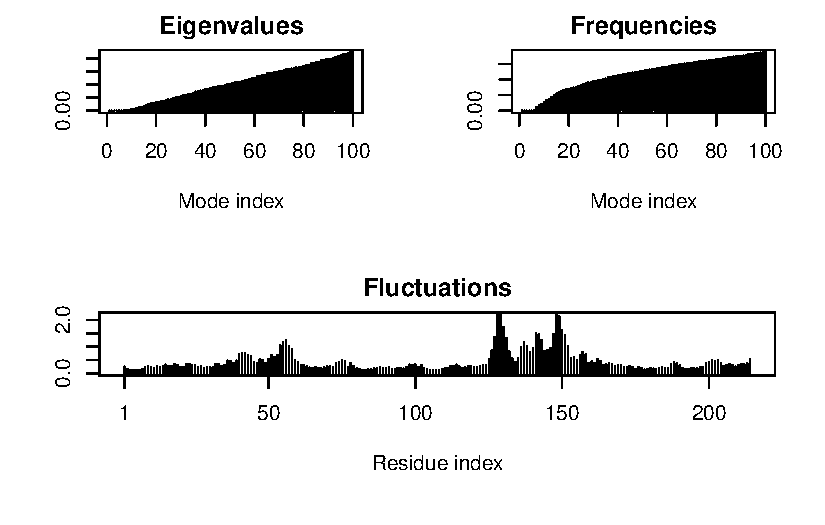
\includegraphics{NLclass09_files/figure-pdf/unnamed-chunk-21-1.pdf}

Write out multi-model PDB file that we can use to make an animation of
the predicted motions.

\begin{Shaded}
\begin{Highlighting}[]
\FunctionTok{mktrj}\NormalTok{(m, }\AttributeTok{file=}\StringTok{"adk.pdb"}\NormalTok{)}
\end{Highlighting}
\end{Shaded}

I can open this in Mol* to play the trajectory\ldots{}




\end{document}
